\documentclass[doublecol]{../macros/epl2} 
% or \documentclass[page-classic]{epl2} for one column style

\title{Measurement of proton-proton elastic scattering and total cross-section at $\sqrt s = 7\,\rm TeV$}
\shorttitle{Title} %Insert here a short version of the title if it exceeds 70 characters

\author{F. Author\inst{1,2} \and S. Author\inst{1} \and T. Author\inst{2}}
\shortauthor{F. Author \etal}

\institute{                    
  \inst{1} First Institute - Address\\
  \inst{2} Second Institute - Address
}
\pacs{13.60.Hb}{Total and inclusive cross sections (including deep-inelastic processes)}


\abstract{
Abstract of the paper.}


\def\d{{\rm d}}
\def\un#1{\,{\rm #1}}
\def\ung#1{\quad({\rm #1})}
\def\unt#1{({\rm #1})}
\def\e{{\rm e}}

\setbox123\hbox{0}
\xdef\S{\hbox to\wd123{\hss}}


\begin{document}

\maketitle

%--------------------------------------------------
\section{Introduction}

TODO: Explain context of this paper, relation to papers 2 and 3.

TODO: Here, we used luminosity from CMS, lumi-independent results will come in paper 3.

TODO: Describe TOTEM - RP, T1, T2; Here only elastic scattering -- only RP -- bridge to the next chapter.


%--------------------------------------------------
\section{Proton measurement with Roman Pots}

\subsection{Roman Pot system}

TODO: Describe the system of RPs: stations, units, ...

TODO: The measurement is performed with the vertical RPs in $220\un{m}$ stations only -- the concept of two diagonals

\subsection{Optics}

TODO: brief description of optics, refer to \cite{epl96} where details are discussed


%--------------------------------------------------
\section{Data taking}

The presented date were recorded during fill 2232 on 10 October 2011, using $\beta^* = 90\un{m}$ optics. For this analysis, only one bunch-pair was used (with populations $5\cdot10^{10}$ and $6\cdot10^{10}$ protons). This bunch-pair produced an instantaneous luminosity dropping from about $6.9$ to $4.3\un{mb^{-1} s^{-1}}$ during the run.

Several trigger schemes were used in the data-taking. For this analysis, the essential one was the RP trigger -- requiring a track-segment in any of the RPs, in at least one of the transverse projections $u$ and $v$, but simultaneously at both arms of the experiment. In order to determine various efficiency corrections, we profited from a zero-bias trigger -- triggering on random bunch-crossings. 

During the run, the Roman Pots (RPs) were driven to three different distances from the beam -- see Tab.~\ref{datasets}. While most of the statistics falls into the first dataset, the other two allowed us to measure $|t|$ values down to $4.6\cdot10^{-3}\un{GeV^2}$. Having three different datasets has enabled us to quantify and reduce certain systematic uncertainties.

\begin{table}
\caption{Description of the three collected datasets. The RP position gives the RP approach to beam in multiples of the beam size ($\sigma_{\rm beam}$). The third column summarizes the numbers of elastic events reconstructed from both diagonals. The $\mathcal{L}_{\rm eff}$ gives the effective (taking into account the DAQ efficiency) luminosity for each dataset. The last column shows the lowest $|t|$ values reached.}
\label{datasets}
\begin{center}
\vskip-3mm
\begin{tabular}{|c|c|c|c|c|}\hline
& RP & elastic                   & $\mathcal{L}_{\rm eff}$ & $|t|_{\rm min}$     \cr
\omit\hss\vbox to 0pt{\vss\hbox{\ dataset\ }\vss}\hss &\multispan4 \cr
 &  position &  events                   & $\unt{mb^{-1}}$         & $\unt{GeV^2}$       \cr\hline
1 & $6.5\,\sigma_{\rm beam}$ & 841k      & $68.2$                  & $7.3\cdot10^{-3}$ \cr
2 & $5.5\,\sigma_{\rm beam}$ & 106k      & $8.2$                   & $5.7\cdot10^{-3}$ \cr
3 & $4.8\,\sigma_{\rm beam}$ & 89k       & $6.6$                   & $4.6\cdot10^{-3}$ \cr\hline
\end{tabular}
\end{center}
\end{table}


%--------------------------------------------------
\section{Analysis}

The analysis is very similar the one of \cite{epl96}. Before we describe all the steps, let us anticipate that all datasets were analyzed separately. Moreover, most of the steps are performed separately on the subsamples coming from the two diagonal topologies (top left -- bottom right and bottom left -- top right). In this way we could control better the systematics of our analysis.

%-------------------------
\subsection{Alignment}

Three complementary methods were applied. First, the RP motor control was calibrated by a beam-touching exercise. Then, proton tracks passing through the overlap between vertical and horizontal RPs were used to determine the relative alignment among the RPs of each unit. Since the elastic event tagging does not require precise alignment, we could use an elastic pre-selection for alignment fine-tuning. By exploiting the azimuthal symmetry of elastic scattering and taking advantage of the very small effective length $L_x$, we could adjust the horizontal and vertical shifts and the tilt of each unit. TODO: residual uncertainties?

%-------------------------
\subsection{Elastic tagging}

The cuts used to select the elastic events are summarized in Tab.~\ref{cuts}. The first two require the reconstructed track collinearity between the left and right arm. The cuts 3-6 effectively work as low-$\xi$ cuts. If $\xi$ is non-negligible, the vertex ($x^*$) reconstruction is broken. So is the correlation between the scattering angle $\theta_y^*$ and the vertical hit difference between far and near RPs. The cut 7 compares the horizontal position reconstructed from the left and right arms. It is the strongest single cut and is very effective against the beam-halo background, see Fig.~\ref{hit dist}.

\begin{table}
\caption{The elastic selection cuts. TODO: add sigmas? The super scripts R and L refer to the right and left arm. Similarly the N and F corresponds to near and far units. TODO: add diagonal (4 tracks out of 4) cut as number 0?}
\label{cuts}
\begin{center}
\begin{tabular}{cc}\hline
1 & $\theta_x^{*\rm R}$ vs. $\theta_x^{*\rm L}$			\cr
2 & $\theta_y^{*\rm R}$ vs. $\theta_y^{*\rm L}$			\cr
3 & $|x^{*\rm R}|$ 									\cr
4 & $|x^{*\rm L}|$ 									\cr
5 & $\theta_y^{*\rm R}$ vs. $y^{\rm R,F} - y^{\rm R,N}$	\cr
6 & $\theta_y^{*\rm L}$ vs. $y^{\rm L,F} - y^{\rm L,N}$	\cr
7 & $x^{*\rm R}$ vs. $x^{*\rm L}$					\cr\hline
\end{tabular}
\end{center}
\end{table}


%-------------------------
\subsection{Kinematics reconstruction}

The scattering angles were reconstructed as in \cite{epl96} -- vertical angle ($\theta^*_y$) from hit position ($y$) and horizontal angle ($\theta^*_x$) from local track angle at a station:
\begin{equation}
\label{reconstruction}
\theta^*_y = {y\over L_y}\ ,\qquad
\theta^*_x = {1\over {\d L_x\over \d s}} \left( \theta_x - {\d v_x\over \d s} x^* \right)\ .
\end{equation}
This is the way that minimizes the influence of optics perturbations (TODO: reference).

TODO: Mention the optics uncertainties? Relevant for systematics evaluation.


%-------------------------
\subsection{Background}

The background contribution (i.e. all non-elastic events passing the selection cuts) was estimated by relaxing the strongest single cut (number 7) and analyzing the distribution of $x^{*\rm R} - x^{*\rm L}$. This distribution can be reasonable described by two Gaussians -- one for the signal and for the background. We determined the background/signal ratio to be $(0.8 \pm 0.4)\%$.

%-------------------------
\subsection{Acceptance correction}

There were two acceptance limitations: the detector edge (relevant for lower $|t|$) and the LHC aperture limitation shown in Fig.~\ref{hit dist} right (relevant for higher $|t|$). Both limitations were treated by assuming azimuthal symmetry and by correcting for smearing around the limitation edges.

%-------------------------
\subsection{Unfolding of resolution effects}

The angular resolution was determined by comparing the scattering angles reconstructed from the left and right arm. Combining all three datasets and all diagonals yields one-arm resolutions $(6.36\pm 0.21)\un{\mu rad}$ in $\theta^*_x$ and $(2.47\pm 0.07)\un{\mu rad}$ in $\theta^*_y$. The latter one is predominantly given by the beam-divergence, the $\theta^*_x$ resolution is deteriorated by a contribution from the finite detector pitch. The resolution impact on the $t$-distribution was determined (and removed) by an iterative procedure. That starts by taking the observed (smeared) $t$-distribution as an input to a Monte-Carlo calculation of the smearing correction. The correction is applied to the observed $t$-distribution which yields a better estimate of the true $t$-distribution. In total, three iterations were made.

%-------------------------
\subsection{Efficiencies}

The efficiency of the RP trigger was estimated from the zero-bias data stream. We selected the elastic events in that stream and found that the RP trigger flag was on each time. Therefore, with $68\%$ confidence level, we concluded the trigger efficiency to be higher than $99.77\%$.
% 95% CL: 99.40

The DAQ efficiency was determined by comparing the numbers of triggered and recorded events, yielding $(98.142 \pm 0.001)\%$.

There are several reasons for reconstruction inefficiency: intrinsic RP detection inefficiency of each silicon sensor, proton interaction with the material of a RP and ``pile-up'' of several protons in one event (RPs can fully reconstruct at most one track). For the last case, the most important situation is a coincidence of an elastic proton and a beam-halo proton, see Fig.~\ref{hit dist}.

Uncorrelated inefficiencies of single RPs were studied by removing the examined RP from the selection cuts (only cut 2 can be kept then) and counting the recuperated events. The result of this study was an inefficiency of $(1.5 \pm 0.2)\%$ for the near and $(3.0 \pm 0.2)\%$ for the far RPs. This difference can be explained by proton interactions in the near pot thus affecting the far RP too. This near-far correlated inefficiency can be determined ... TODO: result, confirmation from MC simulations.

The ``pile-up'' inefficiency was determined from the zero-bias data stream by evaluating the probability of finding a track in both RPs on either side. This probability was increasing as RPs approached the beam. For instance, for the diagonal bottom-left top-right, the probabilities were $(3.9 \pm 0.4)\%$, $(6.2 \pm 0.9)\%$ and $(7.9 \pm 1.1)\%$ for the datasets 1, 2 and 3 respectively.


\begin{figure*}
\begin{center}
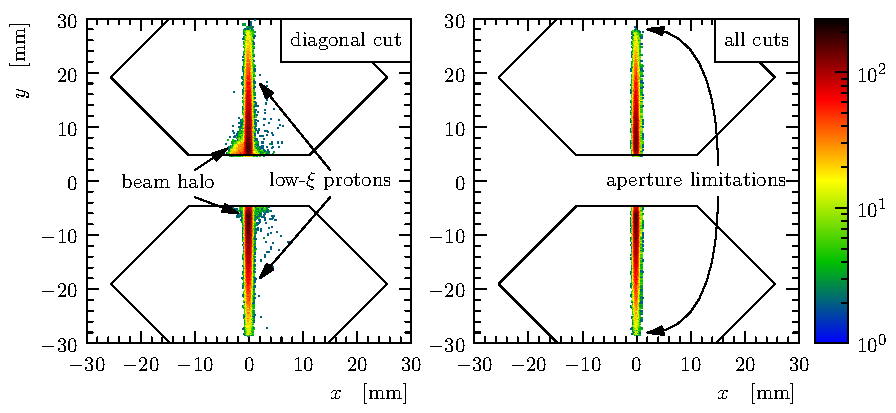
\includegraphics{fig/hit_dist.pdf}
\vskip-5mm
\caption{Hit distributions from dataset 3 in the far unit of the $220\un{m}$ station, right arm. Left: with diagonal cut only, Right: with all the elastic selection cuts (see Tab.~\ref{cuts}). The left plot clearly indicates the presence of the beam halo, which is eliminated by the selection cuts (the right plot). The distribution of elastic hits in right plot is sharply cut at about $|y| = 29\un{mm}$ which is a consequence of the LHC aperture limitations. }
\label{hit dist}
\end{center}
\end{figure*}

%-------------------------
\subsection{Normalization, luminosity}

TODO: Lumi from CMS, 4\% uncertainty, Ken's pedestal subtraction

\subsection{Extrapolation to $t=0\,\rm GeV^2$}

The elastic differential cross section was extrapolated to zero with the following parameterization:
\begin{equation}
\label{extrapolation}
{\d\sigma_{\rm el}\over \d t} = \left. {\d\sigma_{\rm el}\over \d t}\right|_{t=0} \ \e^{-B|t|}\ .
\end{equation}
The fits were performed from the lowest accessible $|t|$ values (see $|t|_{\rm min}$ in Tab.~\ref{datasets}) to $|t| = 0.2\un{GeV^2}$, with a typical $\chi^2/\hbox{n.d.f.}$ of $1.2$ -- see for example the green line in the bottom plot of Fig.~\ref{dsdt}.

%-------------------------
\section{Uncertainty calculation}

TODO: Statistical uncertainty negligible, see Tab.~\ref{results}.

For each of the analysis steps above, the systematic uncertainty was determined, and their combination was studied with a Monte-Carlo simulation. We treated separately analysis $t$-dependent, analysis $t$-independent (normalization) and luminosity uncertainties, the results are shown in the top plot of Fig.~\ref{dsdt}. Since there is a number of contributions in each category, we combined the uncertainties in quadrature. So we did for the total uncertainty.

The luminosity uncertainty is the leading systematic effect for $|t| < 0.2\un{GeV^2}$, above that it is the uncertainty of $\d L_x/\d s$ which dominates.The optics-related error contribution is almost vanishing around $|t| = 0.06\un{GeV^2}$ and has opposite signs left and right of that point. Therefore there is a partial error cancellation in the integrated elastic cross section. Consequently the relative error of $\sigma_{\rm el}$ is significantly lower than the one of $\d\sigma_{\rm el}/\d t|_0$ -- see Tab.~\ref{results}.

The Monte-Carlo simulation confirms that there is a strong correlation between the errors of $\sigma_{\rm el}$ and $\d\sigma_{\rm el}/\d t|_0$ -- the correlation coefficient is $0.76$ (when both $t$-dependent and normalization contributions are included).



%--------------------------------------------------
\section{Results}

\subsection{$t$-distribution}

TODO: very good agreement among datasets and diagonals

Shown in Fig.~\ref{dsdt}, data presented in Tab.~\ref{data low t} and in Tab.~\ref{data medium t}.

TODO: how the bin control points were calculated -- why there is no $t$ error in Tab.~\ref{data low t}

%\begin{figure*}
%\begin{center}
%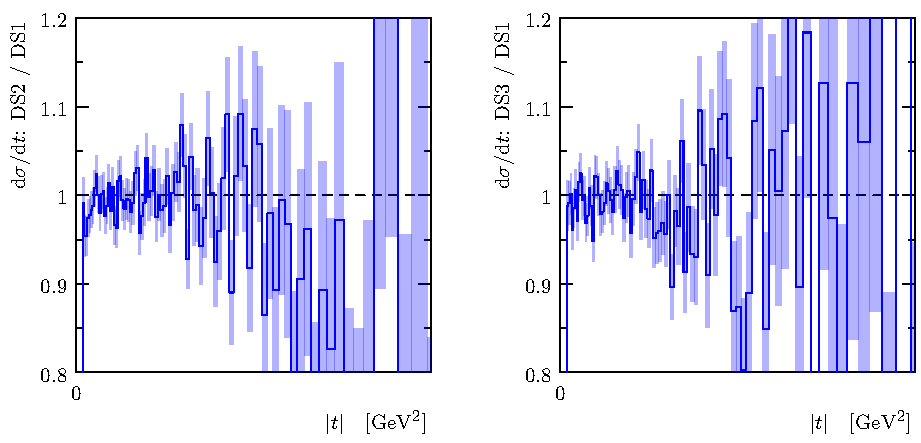
\includegraphics{fig/dsdt_dataset_ratio.pdf}
%\caption{A figure that demonstrates the excelent match between the data-sets.}
%\label{f.lbl}
%\end{center}
%\end{figure*}


\begin{table}
\caption{Low $|t|$ data results, $\beta^* = 90\un{m}$, this analysis. Statistical errors only.}
\label{data low t}
\begin{center}
\vskip-3mm
\begin{tabular}{|c|c|c|c|c|}
\multispan2\hrulefill &\omit &\multispan2\hrulefill\cr
$|t|$ & $\d \sigma_{\rm el}/\d t$ &\omit\ \vrule& $|t|$ & $\d \sigma_{\rm el}/\d t$\cr
$\unt{GeV^2}$ & $\unt{mb/GeV^2}$ &\omit\ \vrule& $\unt{GeV^2}$ & $\unt{mb/GeV^2}$\cr
\multispan2\hrulefill &\omit &\multispan2\hrulefill\cr
$0.00515$ & $465.\S\S \pm 27.\S\S$ &\omit\ \vrule& $0.112$ & $\S54.11\S \pm 0.53\S$\cr
$0.00650$ & $465.\S\S \pm 11.\S\S$ &\omit\ \vrule& $0.116$ & $\S51.21\S \pm 0.51\S$\cr
$0.00818$ & $437.5\S \pm \S5.0\S$ &\omit\ \vrule& $0.119$ & $\S48.24\S \pm 0.49\S$\cr
$0.00995$ & $411.0\S \pm \S3.3\S$ &\omit\ \vrule& $0.122$ & $\S44.99\S \pm 0.46\S$\cr
$0.0117\S$ & $402.3\S \pm \S2.9\S$ &\omit\ \vrule& $0.126$ & $\S42.74\S \pm 0.45\S$\cr
$0.0135\S$ & $384.5\S \pm \S2.6\S$ &\omit\ \vrule& $0.130$ & $\S39.49\S \pm 0.43\S$\cr
$0.0154\S$ & $378.0\S \pm \S2.4\S$ &\omit\ \vrule& $0.133$ & $\S35.75\S \pm 0.43\S$\cr
$0.0172\S$ & $360.3\S \pm \S2.3\S$ &\omit\ \vrule& $0.137$ & $\S33.63\S \pm 0.41\S$\cr
$0.0191\S$ & $348.1\S \pm \S2.2\S$ &\omit\ \vrule& $0.141$ & $\S31.08\S \pm 0.41\S$\cr
$0.0210\S$ & $337.0\S \pm \S2.1\S$ &\omit\ \vrule& $0.145$ & $\S28.91\S \pm 0.39\S$\cr
$0.0229\S$ & $325.0\S \pm \S2.0\S$ &\omit\ \vrule& $0.149$ & $\S25.65\S \pm 0.38\S$\cr
$0.0248\S$ & $307.9\S \pm \S1.9\S$ &\omit\ \vrule& $0.153$ & $\S24.16\S \pm 0.36\S$\cr
$0.0268\S$ & $296.7\S \pm \S1.8\S$ &\omit\ \vrule& $0.157$ & $\S22.35\S \pm 0.35\S$\cr
$0.0287\S$ & $285.9\S \pm \S1.8\S$ &\omit\ \vrule& $0.162$ & $\S20.22\S \pm 0.34\S$\cr
$0.0307\S$ & $275.3\S \pm \S1.7\S$ &\omit\ \vrule& $0.166$ & $\S19.01\S \pm 0.32\S$\cr
$0.0328\S$ & $263.0\S \pm \S1.6\S$ &\omit\ \vrule& $0.171$ & $\S16.92\S \pm 0.30\S$\cr
$0.0348\S$ & $252.0\S \pm \S1.6\S$ &\omit\ \vrule& $0.175$ & $\S15.20\S \pm 0.29\S$\cr
$0.0369\S$ & $242.8\S \pm \S1.5\S$ &\omit\ \vrule& $0.180$ & $\S13.90\S \pm 0.28\S$\cr
$0.0390\S$ & $231.6\S \pm \S1.5\S$ &\omit\ \vrule& $0.185$ & $\S12.09\S \pm 0.26\S$\cr
$0.0411\S$ & $222.2\S \pm \S1.4\S$ &\omit\ \vrule& $0.190$ & $\S11.26\S \pm 0.25\S$\cr
$0.0433\S$ & $210.9\S \pm \S1.4\S$ &\omit\ \vrule& $0.196$ & $\S10.11\S \pm 0.23\S$\cr
$0.0455\S$ & $204.8\S \pm \S1.3\S$ &\omit\ \vrule& $0.201$ & $\S\S9.31\S \pm 0.22\S$\cr
$0.0477\S$ & $197.2\S \pm \S1.3\S$ &\omit\ \vrule& $0.207$ & $\S\S8.07\S \pm 0.21\S$\cr
$0.0499\S$ & $187.5\S \pm \S1.3\S$ &\omit\ \vrule& $0.213$ & $\S\S6.98\S \pm 0.19\S$\cr
$0.0522\S$ & $178.1\S \pm \S1.2\S$ &\omit\ \vrule& $0.219$ & $\S\S6.22\S \pm 0.17\S$\cr
$0.0545\S$ & $168.8\S \pm \S1.2\S$ &\omit\ \vrule& $0.225$ & $\S\S5.38\S \pm 0.16\S$\cr
$0.0569\S$ & $162.5\S \pm \S1.1\S$ &\omit\ \vrule& $0.232$ & $\S\S4.40\S \pm 0.14\S$\cr
$0.0592\S$ & $155.5\S \pm \S1.1\S$ &\omit\ \vrule& $0.239$ & $\S\S4.25\S \pm 0.14\S$\cr
$0.0616\S$ & $149.4\S \pm \S1.1\S$ &\omit\ \vrule& $0.246$ & $\S\S3.47\S \pm 0.13\S$\cr
$0.0641\S$ & $140.2\S \pm \S1.0\S$ &\omit\ \vrule& $0.253$ & $\S\S2.82\S \pm 0.11\S$\cr
$0.0666\S$ & $135.10 \pm \S0.99$ &\omit\ \vrule& $0.261$ & $\S\S2.52\S \pm 0.10\S$\cr
$0.0691\S$ & $129.00 \pm \S0.96$ &\omit\ \vrule& $0.270$ & $\S\S2.142 \pm 0.097$\cr
$0.0716\S$ & $120.53 \pm \S0.91$ &\omit\ \vrule& $0.278$ & $\S\S1.824 \pm 0.086$\cr
$0.0742\S$ & $115.10 \pm \S0.89$ &\omit\ \vrule& $0.287$ & $\S\S1.455 \pm 0.075$\cr
$0.0769\S$ & $109.63 \pm \S0.86$ &\omit\ \vrule& $0.297$ & $\S\S1.257 \pm 0.069$\cr
$0.0795\S$ & $104.97 \pm \S0.83$ &\omit\ \vrule& $0.307$ & $\S\S0.848 \pm 0.055$\cr
$0.0823\S$ & $100.22 \pm \S0.80$ &\omit\ \vrule& $0.318$ & $\S\S0.633 \pm 0.046$\cr
$0.0850\S$ & $\S93.18 \pm \S0.76$ &\omit\ \vrule& $0.330$ & $\S\S0.558 \pm 0.043$\cr
$0.0878\S$ & $\S89.16 \pm \S0.74$ &\omit\ \vrule& $0.342$ & $\S\S0.417 \pm 0.038$\cr
$0.0907\S$ & $\S81.78 \pm \S0.70$ &\omit\ \vrule& $0.356$ & $\S\S0.269 \pm 0.027$\cr
$0.0936\S$ & $\S78.85 \pm \S0.68$ &\omit\ \vrule& $0.371$ & $\S\S0.235 \pm 0.025$\cr
$0.0966\S$ & $\S73.92 \pm \S0.65$ &\omit\ \vrule& $0.387$ & $\S\S0.136 \pm 0.019$\cr
$0.0996\S$ & $\S68.77 \pm \S0.62$ &\omit\ \vrule& $0.405$ & $\S\S0.109 \pm 0.016$\cr
$0.103\S\S$ & $\S65.53 \pm \S0.60$ &\omit\ \vrule& $0.425$ & $\S\S0.058 \pm 0.011$\cr
$0.106\S\S$ & $\S61.90 \pm \S0.58$ &\omit\ \vrule& $0.448$ & $\S\S0.029 \pm 0.007$\cr
\multispan2 &\omit &\multispan2\hrulefill\cr
$0.109\S\S$ & $\S58.11 \pm \S0.55$\cr
\multispan2\hrulefill &\omit &\multispan2\cr
\end{tabular}
\end{center}
\end{table}

\begin{table}
\caption{Medium $|t|$ data results, $\beta^* = 3.5\un{m}$, Ref.~\cite{epl95}. NOT FINAL - just a place-holder.}
\label{data medium t}
\begin{center}
\vskip-3mm
\begin{tabular}{|c|c|c|c|c|c|c|c|}\hline
$|t|$ & $\d \sigma_{\rm el}/\d t$ &\omit\ \vrule& $|t|$ & $\d \sigma_{\rm el}/\d t$\cr
$\unt{GeV^2}$ & $\unt{\mu b/GeV^2}$ &\omit\ \vrule& $\unt{GeV^2}$ & $\unt{\mu b/GeV^2}$\cr\hline
$ 0.3643 \pm 0.0032 $ & $ 299.2\S \pm 6.9\S $  &\omit\ \vrule& $ 0.8310 \pm 0.0078 $ & $ \S18.93\S\S \pm 0.71\S\S $\cr
$ 0.3707 \pm 0.0032 $ & $ 251.8\S \pm 5.8\S $  &\omit\ \vrule& $ 0.8467 \pm 0.0079 $ & $ \S18.32\S\S \pm 0.68\S\S $\cr
$ 0.3773 \pm 0.0033 $ & $ 225.1\S \pm 5.1\S $  &\omit\ \vrule& $ 0.8629 \pm 0.0083 $ & $ \S16.33\S\S \pm 0.62\S\S $\cr
$ 0.3840 \pm 0.0033 $ & $ 174.3\S \pm 4.2\S $  &\omit\ \vrule& $ 0.8797 \pm 0.0085 $ & $ \S16.42\S\S \pm 0.61\S\S $\cr
$ 0.3908 \pm 0.0035 $ & $ 157.1\S \pm 3.8\S $  &\omit\ \vrule& $ 0.8966 \pm 0.0084 $ & $ \S16.95\S\S \pm 0.63\S\S $\cr
$ 0.3978 \pm 0.0035 $ & $ 133.3\S \pm 3.2\S $  &\omit\ \vrule& $ 0.9134 \pm 0.0084 $ & $ \S14.14\S\S \pm 0.56\S\S $\cr
$ 0.4050 \pm 0.0036 $ & $ 116.1\S \pm 2.9\S $  &\omit\ \vrule& $ 0.9306 \pm 0.0088 $ & $ \S14.05\S\S \pm 0.55\S\S $\cr
$ 0.4124 \pm 0.0038 $ & $ \S92.6\S \pm 2.4\S $  &\omit\ \vrule& $ 0.9482 \pm 0.0088 $ & $ \S14.10\S\S \pm 0.56\S\S $\cr
$ 0.4200 \pm 0.0039 $ & $ \S78.1\S \pm 2.1\S $  &\omit\ \vrule& $ 0.9663 \pm 0.0093 $ & $ \S11.91\S\S \pm 0.48\S\S $\cr
$ 0.4280 \pm 0.0040 $ & $ \S63.2\S \pm 1.7\S $  &\omit\ \vrule& $ 0.9853 \pm 0.0097 $ & $ \S12.24\S\S \pm 0.48\S\S $\cr
$ 0.4363 \pm 0.0042 $ & $ \S53.6\S \pm 1.5\S $  &\omit\ \vrule& $ 1.0048 \pm 0.0098 $ & $ \S11.31\S\S \pm 0.46\S\S $\cr
$ 0.4450 \pm 0.0045 $ & $ \S44.7\S \pm 1.3\S $  &\omit\ \vrule& $ 1.0243 \pm 0.0098 $ & $ \S10.04\S\S \pm 0.43\S\S $\cr
$ 0.4542 \pm 0.0047 $ & $ \S33.7\S \pm 1.1\S $  &\omit\ \vrule& $ 1.044\S \pm 0.010\S $ & $ \S\S8.73\S\S \pm 0.39\S\S $\cr
$ 0.4639 \pm 0.0050 $ & $ \S30.25 \pm 0.98 $  &\omit\ \vrule& $ 1.065\S \pm 0.011\S $ & $ \S\S7.87\S\S \pm 0.36\S\S $\cr
$ 0.4742 \pm 0.0053 $ & $ \S25.54 \pm 0.85 $  &\omit\ \vrule& $ 1.086\S \pm 0.011\S $ & $ \S\S8.13\S\S \pm 0.36\S\S $\cr
$ 0.4849 \pm 0.0054 $ & $ \S21.58 \pm 0.75 $  &\omit\ \vrule& $ 1.109\S \pm 0.011\S $ & $ \S\S7.20\S\S \pm 0.34\S\S $\cr
$ 0.4960 \pm 0.0057 $ & $ \S19.44 \pm 0.70 $  &\omit\ \vrule& $ 1.131\S \pm 0.012\S $ & $ \S\S6.50\S\S \pm 0.31\S\S $\cr
$ 0.5077 \pm 0.0060 $ & $ \S18.04 \pm 0.66 $  &\omit\ \vrule& $ 1.155\S \pm 0.012\S $ & $ \S\S5.09\S\S \pm 0.26\S\S $\cr
$ 0.5201 \pm 0.0065 $ & $ \S17.06 \pm 0.63 $  &\omit\ \vrule& $ 1.180\S \pm 0.013\S $ & $ \S\S5.26\S\S \pm 0.26\S\S $\cr
$ 0.5332 \pm 0.0066 $ & $ \S16.07 \pm 0.62 $  &\omit\ \vrule& $ 1.206\S \pm 0.013\S $ & $ \S\S4.96\S\S \pm 0.25\S\S $\cr
$ 0.5465 \pm 0.0067 $ & $ \S16.85 \pm 0.66 $  &\omit\ \vrule& $ 1.233\S \pm 0.014\S $ & $ \S\S4.22\S\S \pm 0.22\S\S $\cr
$ 0.5601 \pm 0.0069 $ & $ \S18.46 \pm 0.72 $  &\omit\ \vrule& $ 1.261\S \pm 0.015\S $ & $ \S\S3.40\S\S \pm 0.19\S\S $\cr
$ 0.5739 \pm 0.0068 $ & $ \S18.26 \pm 0.72 $  &\omit\ \vrule& $ 1.291\S \pm 0.015\S $ & $ \S\S3.26\S\S \pm 0.18\S\S $\cr
$ 0.5877 \pm 0.0070 $ & $ \S20.77 \pm 0.79 $  &\omit\ \vrule& $ 1.322\S \pm 0.016\S $ & $ \S\S2.69\S\S \pm 0.16\S\S $\cr
$ 0.6016 \pm 0.0070 $ & $ \S22.85 \pm 0.85 $  &\omit\ \vrule& $ 1.355\S \pm 0.017\S $ & $ \S\S2.21\S\S \pm 0.14\S\S $\cr
$ 0.6155 \pm 0.0069 $ & $ \S22.23 \pm 0.85 $  &\omit\ \vrule& $ 1.390\S \pm 0.019\S $ & $ \S\S2.00\S\S \pm 0.13\S\S $\cr
$ 0.6293 \pm 0.0070 $ & $ \S24.23 \pm 0.90 $  &\omit\ \vrule& $ 1.428\S \pm 0.019\S $ & $ \S\S1.63\S\S \pm 0.11\S\S $\cr
$ 0.6433 \pm 0.0071 $ & $ \S24.65 \pm 0.90 $  &\omit\ \vrule& $ 1.467\S \pm 0.020\S $ & $ \S\S1.47\S\S \pm 0.11\S\S $\cr
$ 0.6572 \pm 0.0069 $ & $ \S27.43 \pm 0.97 $  &\omit\ \vrule& $ 1.508\S \pm 0.021\S $ & $ \S\S1.066\S \pm 0.086\S $\cr
$ 0.6711 \pm 0.0070 $ & $ \S24.79 \pm 0.91 $  &\omit\ \vrule& $ 1.553\S \pm 0.025\S $ & $ \S\S0.841\S \pm 0.070\S $\cr
$ 0.6853 \pm 0.0071 $ & $ \S25.11 \pm 0.91 $  &\omit\ \vrule& $ 1.604\S \pm 0.026\S $ & $ \S\S0.747\S \pm 0.065\S $\cr
$ 0.6995 \pm 0.0072 $ & $ \S27.35 \pm 0.94 $  &\omit\ \vrule& $ 1.658\S \pm 0.028\S $ & $ \S\S0.557\S \pm 0.054\S $\cr
$ 0.7136 \pm 0.0069 $ & $ \S26.52 \pm 0.94 $  &\omit\ \vrule& $ 1.715\S \pm 0.029\S $ & $ \S\S0.464\S \pm 0.047\S $\cr
$ 0.7276 \pm 0.0071 $ & $ \S25.87 \pm 0.91 $  &\omit\ \vrule& $ 1.779\S \pm 0.035\S $ & $ \S\S0.369\S \pm 0.039\S $\cr
$ 0.7420 \pm 0.0073 $ & $ \S25.05 \pm 0.88 $  &\omit\ \vrule& $ 1.853\S \pm 0.039\S $ & $ \S\S0.216\S \pm 0.028\S $\cr
$ 0.7566 \pm 0.0072 $ & $ \S26.03 \pm 0.90 $  &\omit\ \vrule& $ 1.935\S \pm 0.042\S $ & $ \S\S0.192\S \pm 0.025\S $\cr
$ 0.7712 \pm 0.0074 $ & $ \S24.07 \pm 0.85 $  &\omit\ \vrule& $ 2.027\S \pm 0.051\S $ & $ \S\S0.126\S \pm 0.018\S $\cr
$ 0.7860 \pm 0.0074 $ & $ \S23.16 \pm 0.81 $  &\omit\ \vrule& $ 2.138\S \pm 0.060\S $ & $ \S\S0.059\S \pm 0.011\S $\cr
$ 0.8008 \pm 0.0073 $ & $ \S21.34 \pm 0.78 $  &\omit\ \vrule& $ 2.282\S \pm 0.085\S $ & $ \S\S0.0412 \pm 0.0083 $\cr
$ 0.8157 \pm 0.0076 $ & $ \S21.59 \pm 0.77 $  &\omit\ \vrule& $ 2.455\S \pm 0.088\S $ & $ \S\S0.0230 \pm 0.0055 $\cr\hline
\end{tabular}
\end{center}
\end{table}


\begin{figure*}
\begin{center}
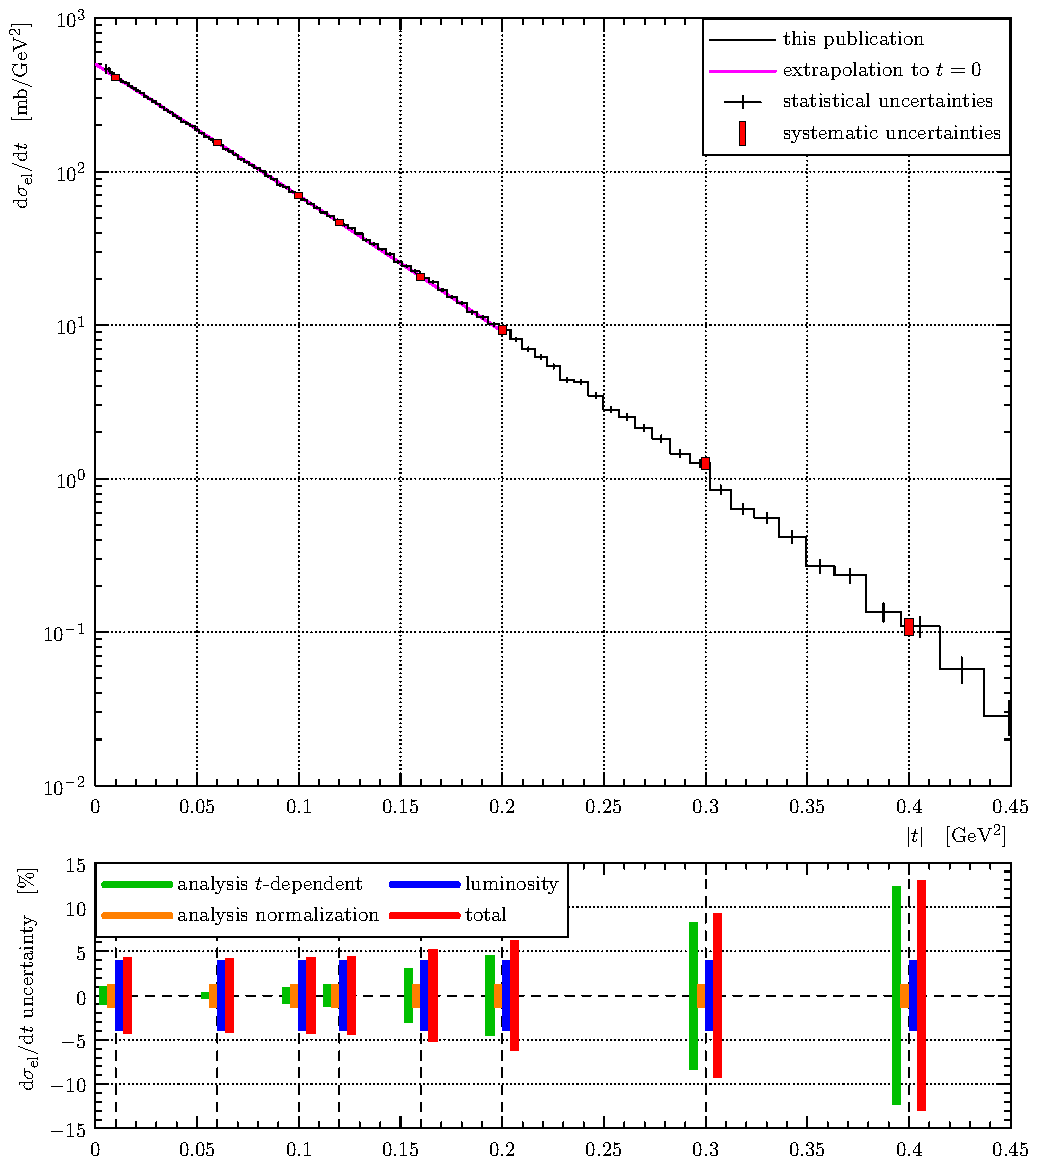
\includegraphics{fig/dsdt.pdf}
\caption{The measured elastic differential cross section (bottom plot) with systematic uncertainty estimation (upper plot). TODO: more details}
\label{dsdt}
\end{center}
\end{figure*}





\subsection{Cross sections -- need better name}

TODO: Comment on the reducing ration of extrapolated/observed $\sigma_{el}$


TODO: Ref to Tab.~\ref{results}

\begin{largetable}
\caption{Result summary. The right-most column gives the total systematic uncertainty, combined in quadrature and taking into account the correlations between the contributions.}
\vskip-3mm
\label{results}
\begin{tabular}{cccccccl}\hline
quantity & value & statistical u. &\multispan5\hss systematic uncertainty\hss\cr\hline
%
$\d\sigma_{\rm el}/\d t|_0$ & $506.4\un{mb/GeV^2}$ & $\pm 0.2\%^{\rm stat}$ & $\pm 1.7\%^{t-\rm dep}$ & $\pm 1.3\%^{\rm norm}$ & $\pm 4\%^{\rm lumi}$ &  & $\Rightarrow \pm 4.5\%^{\rm syst}$\cr
%
$B$ & $19.89\un{GeV^{-2}}$ & $\pm 0.03\%^{\rm stat}$  & $\pm 0.27\%^{\rm t-dep}$ & & & & $ \Rightarrow \pm 0.27\%^{\rm syst}$\cr
%
$\sigma_{\rm el}$ & $25.43\un{mb}$ & $\pm 0.1\%^{\rm stat}$ & $\pm 0.4\%^{t-\rm dep}$ & $\pm 1.3\%^{\rm norm}$ & $\pm 4\%^{\rm lumi}$ &  & $\Rightarrow \pm 4.2\%^{\rm syst}$\cr\hline
%
$\sigma_{\rm tot}$ & $98.6\un{mb}$ & & $\pm 0.85\%^{\rm t-dep}$ & $\pm 0.65\%^{\rm norm}$ & $\pm 2.0\%^{\rm lumi}$ & $^{+1.14}_{-0.14} \%^{\rm rho}$ & $ \Rightarrow ^{+2.45}_{-2.19} \%^{\rm syst}$\cr
%
$\sigma_{\rm inel}$ & $73.2\un{mb}$ & & $\pm 1.05\%^{\rm t-dep}$ & $\pm 0.42\%^{\rm norm}$ & $\pm 1.3\%^{\rm lumi}$ & $^{+1.54}_{-0.19} \%^{\rm rho}$ & $ \Rightarrow ^{+3.26}_{-2.90} \%^{\rm syst}$\cr\hline
\end{tabular}
\end{largetable}



\begin{equation}
\label{si tot}
\sigma_{\rm tot} = {16\pi (\hbar c)^2\over 1 + \rho^2}\, {\d N_{\rm el}/\d t|_0\over N_{\rm el} + N_{\rm inel}}\ ,\qquad
\sigma_{\rm inel} = \sigma_{\rm tot} - \sigma_{\rm el}
\end{equation}


%--------------------------------------------------
\section{Conclusions and outlook}

TODO: results consistent among all datasets and agree well with \cite{epl96}

TODO: for $4.6\cdot10^{-3}\un{GeV^2} < |t| < 0.2\un{GeV^2}$ there is no indication for differential slope variation

TODO: compared to \cite{epl96}, better extrapolation -- smaller ratio of extrapolated/observed regions

TODO: $\sigma_{\rm inel}$: here inclusively, individual components will be given later -- bridge to paper 2 and future publications

TODO: increasing $B$ -- $t$-distribution shrinking -- protons grow with $\sqrt s$

TODO: $\sigma_{\rm el} / \sigma_{\rm inel}$ -- indicates the ``shape'' of the proton; need interpretation for the ratio growing with $\sqrt s$

TODO: planning to repeat the measurement at $\sqrt s = 8\un{TeV}$



\begin{figure}
\onefigure{fig/B_s.pdf}
\caption{Figure caption.}
\label{fig.1}
\end{figure}

\begin{figure}
\onefigure{fig/sigma_el_to_sigma_tot.pdf}
\caption{Figure caption.}
\label{fig.1}
\end{figure}




%--------------------------------------------------
\acknowledgments
Acknowledgements -- Insert here the text.


%--------------------------------------------------
\begin{thebibliography}{0}

\bibitem{epl96}
    %First measurements of the total proton-proton cross section at the LHC energy of $\sqrt s =7\,\rm TeV$ CERN-PH-EP-2011-158
	\Name{Antchev G.~et al.~(TOTEM Collaboration)}
	\REVIEW{Europhys.~Lett.}{96}{2011}{21002}

\bibitem{epl95}
    %Proton-proton elastic scattering at the LHC energy of \sqrt{s} = 7 TeV, Europhys. Lett. 95 (2011) 41001,CERN-PH-EP-2011-101 
	\Name{Antchev G.~et al.~(TOTEM Collaboration)}
	\REVIEW{Europhys.~Lett.}{95}{2011}{41001}

\bibitem{jinst}
    %The TOTEM Experiment at the CERN Large Hadron Collider, JINST 3 S08007, 2008
	\Name{Anelli G.~et al.~(TOTEM Collaboration)}
	\REVIEW{JINST}{3}{2008}{S08007}

%\bibitem{b.b}
%  \Name{Author F. \and Author S.}
%  \Book{Some Book of Interest}
%  \Editor{A. Editor}
%  \Vol{9}
%  \Publ{Publishing house, City}
%  \Year{1939}
%  \Page{666}.
%
%\bibitem{b.c}
%  \Editor{Editor A.}
%  \Book{Some Book of Interest}
%  \Vol{9}
%  \Publ{Publishing house, City}
%  \Year{1939}
%  \Section{A}.

\end{thebibliography}

\end{document}
